The data related to each subject and modality were chronologically
juxtaposed exactly in the order the experiments were performed; then a
label was attached to each sample, according to the type of grasp
required from the subject. Samples associated with a low force value
were given the label $0$, since they denote no activity of the
muscles, that is, a resting condition. Subject $1$ actually needed the
no-action data set to be replicated for each modality, since we did
not record its baseline each time --- a mistake which was corrected
with the second and third subject. Moreover, we could not record the
"pointing index" activity for this subject in the second modality,
which is therefore null.

\begin{figure*}[!ht] \centering
  \begin{tabular}{ccc}
    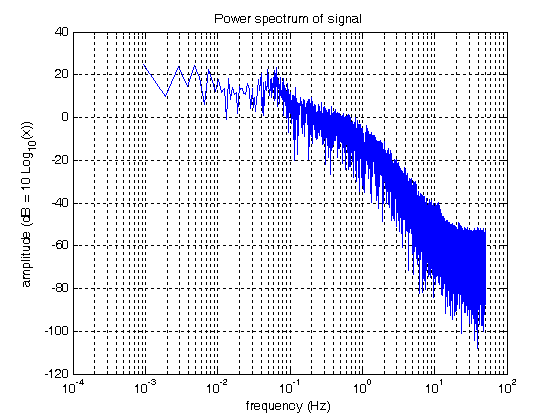
\includegraphics[width=0.3\textwidth]{figs/spectrum_force} &
    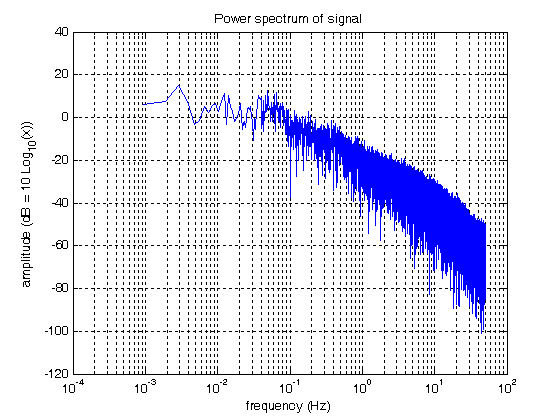
\includegraphics[width=0.3\textwidth]{figs/spectrum_electrode_1} &
    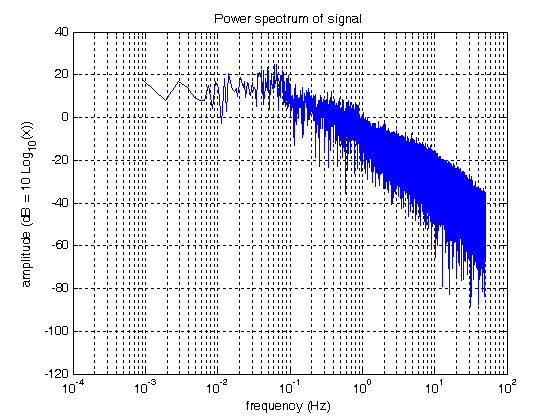
\includegraphics[width=0.3\textwidth]{figs/spectrum_electrode_3} \\
    force & electrode $1$ & electrode $3$ \\
  \end{tabular}
  \caption{frequency analysis of the force signal and two
    typical electrodes.}
  \label{fig:spectra}
\end{figure*}

Spectral analysis of the EMG signal as read from the electrodes, in
agreement with the literature, shows that its relevant bandwidth lies
below $10$-$12$Hz (see Figure \ref{fig:spectra}), so we could safely
subsample the signals at $25$Hz, that is, considering one sample in
four of the original data stream. This made the data set to be dealt
with much smaller and computationally tractable. Subsequently, we
applied a II order low-pass filter with cutoff frequency at $5$Hz in
order to remove all possible high-frequency noise. This has proved to
be a very effective way of getting a good signal in early experiments
(see \cite{2008.Neurorob}).

Principal Component Analysis (PCA) reveals that the 5 signals can be
linearly reduced to two losing, on average, only $7.7\% \pm 4.4\%$ of
the signal variance; therefore, we can visualise the samples, tagging
them according to the labels (and therefore according to the action)
and visually detecting how well the subjects can produce different EMG
patterns when they are asked to simulate different grasping
actions. Figure \ref{fig:PCA} shows the results, according to each
subject and modality.

\begin{figure*}[!ht] \centering
  \begin{tabular}{ccc}
    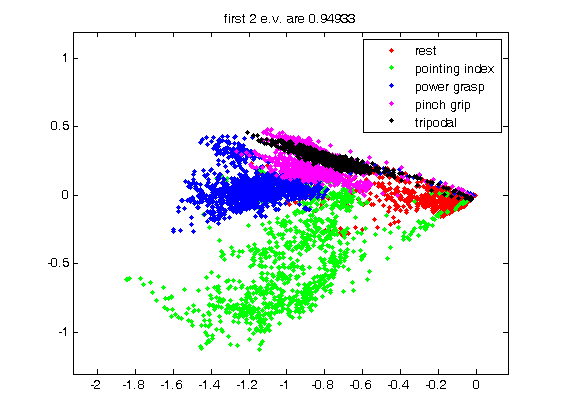
\includegraphics[width=0.3\textwidth]{figs/data11} &
    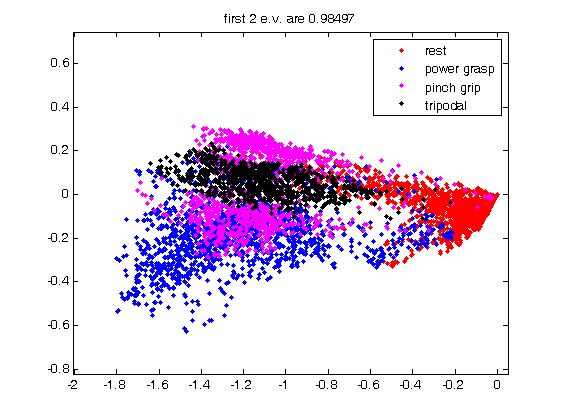
\includegraphics[width=0.3\textwidth]{figs/data12} &
    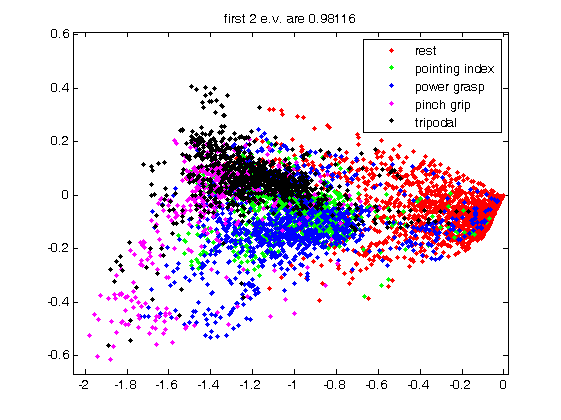
\includegraphics[width=0.3\textwidth]{figs/data13} \\
    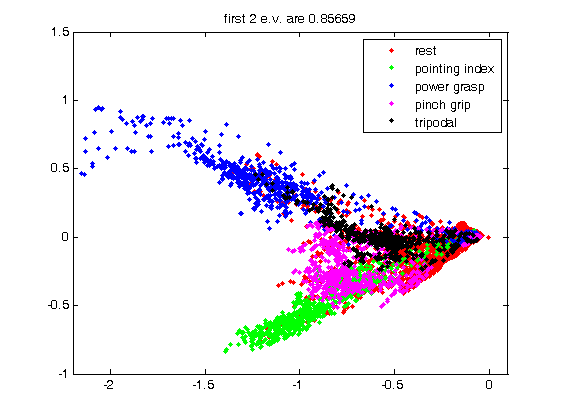
\includegraphics[width=0.3\textwidth]{figs/data21} &
    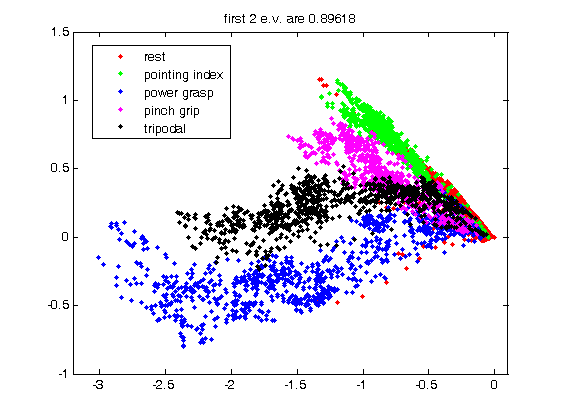
\includegraphics[width=0.3\textwidth]{figs/data22} &
    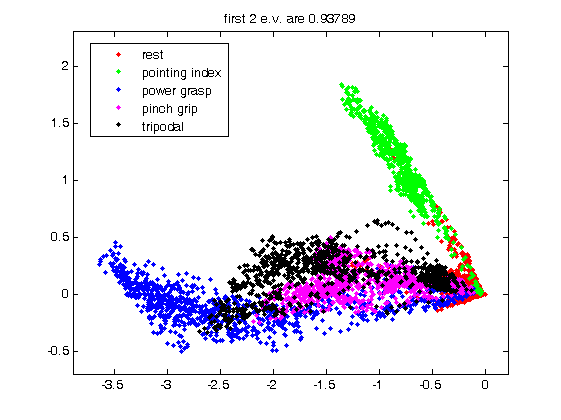
\includegraphics[width=0.3\textwidth]{figs/data23} \\
    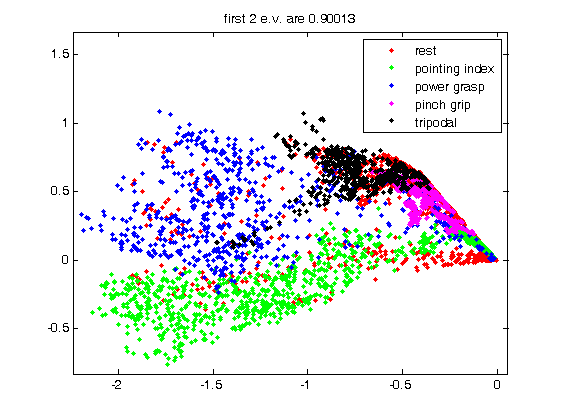
\includegraphics[width=0.3\textwidth]{figs/data31} &
    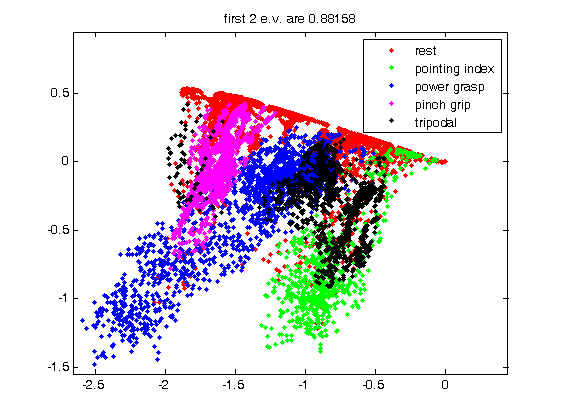
\includegraphics[width=0.3\textwidth]{figs/data32} &
    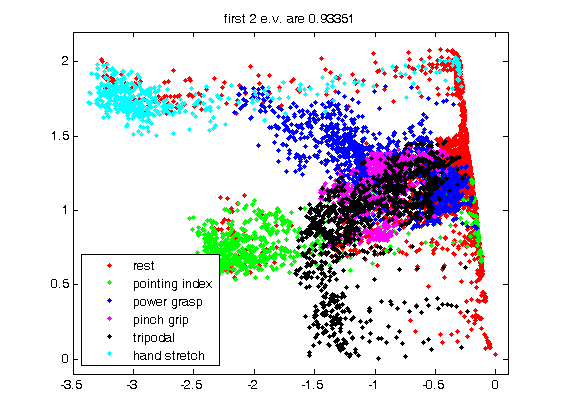
\includegraphics[width=0.3\textwidth]{figs/data33} \\
  \end{tabular}
  \caption{ PCA analysis of the subjects' data. (top to bottom)
    Subject $1$, $2$ and $3$; (left to right) modality $1$, $2$ and
    $3$. Notice that subject $1$, modality $2$ has no ``pointing
    index'' data, and that subject $3$ has the ``hand stretch'' data.}
  \label{fig:PCA}
\end{figure*}

As is apparent from the Figure, all subjects can produce remarkably
well separated and distinct signals, according to the elicited type of
grasp. In particular, notice how two very similar grasp types, i.e.,
pinch grip (thumb and index come together as to precisely grip, e.g.,
a pen) and tripodal grip (the same, but done with the middle finger,
too) appear well separated on almost each graph --- look at the black
and pink coloured samples.

Notice, as well, that the graphs have not all the same scale and that
they appear incongruent with one another, but this is due to
having positioned the electrodes irrespective of their order number on
the stumps of the patients. This is anyway ininfluent, since SVMs
are exaclty supposed to automatically find patterns and regularities
among the samples for each subject.

One last point is that PCA being so effective in reducing the
dimensionality of our data to two does not necessarily imply that we
could use two electrodes only to obtain the same results; this depends
on the PCA coefficients, which show consistently the same magnitude
(except in the case of subject $3$, where a heavy drift was observed
on two electrodes, very likely due to sweating --- this is a well-known
problem of EMG-controlled prosthetics). This means that each electrode
is required to give a uniformly-weighted contribution to the
PCA-transformed $2$-dimensional samples. Of course reducing the
required number of electrodes is a requirement, since this would make
the prosthesis cheaper. We are invesitigating the issue.
